\section{Thực nghiệm và đánh giá kết quả}
\label{sec:thuc-nghiem}

Chương này trình bày kết quả cụ thể của hai giai đoạn trong pipeline, bao gồm kết quả lựa chọn đặc trưng (Phase 1) và kết quả huấn luyện/đánh giá mô hình theo thiết kế Leave-One-Group-Out (Phase 2). Các kết quả số được trích xuất từ notebook \href{https://github.com/hoainn/HocMayATTT/blob/main/phase1\_feature\_selection.ipynb}{\texttt{phase1\_feature\_selection.ipynb}} và \href{https://github.com/hoainn/HocMayATTT/blob/main/phase2\_model\_training.ipynb}{\texttt{phase2\_model\_training.ipynb}}. Sơ đồ chi tiết pipeline đã được trình bày trong Hình~\ref{fig:phase1_diagram} và Hình~\ref{fig:phase2_diagram} (Chương~\ref{sec:phuong-phap}).

\subsection{Kết quả Phase 1: Lựa chọn đặc trưng FAMS}

\subsubsection{So sánh hai ngưỡng bỏ phiếu}

Phase 1 áp dụng khung FAMS với hai ngưỡng bỏ phiếu để xác định tập đặc trưng phù hợp nhất cho Phase 2. Mỗi phương pháp trong 5 phương pháp (Variance, Mutual Information, RFE, Lasso L1, RF Importance) chọn top-25 đặc trưng; hai ngưỡng được so sánh:

\begin{itemize}
    \item \textbf{Votes $\geq 3$:} Đặc trưng được chọn bởi ít nhất 3/5 phương pháp $\to$ \textbf{18 đặc trưng}.
    \item \textbf{Votes $> 3$:} Đặc trưng được chọn bởi ít nhất 4/5 phương pháp $\to$ \textbf{6 đặc trưng}.
\end{itemize}

Bảng~\ref{tab:phase1_eval} so sánh hiệu năng phân loại của ba mô hình trên tập test của bộ Kaggle với hai ngưỡng này.

\begin{table*}[!t]
\caption{So sánh hiệu năng theo ngưỡng bỏ phiếu FAMS trên bộ dữ liệu Kaggle.}
\label{tab:phase1_eval}
\begin{center}
\begin{adjustbox}{width=\textwidth}
\begin{tabular}{|l|l|r|r|r|r|r|r|r|}
\hline
\textbf{Ngưỡng} & \textbf{Mô hình} & \textbf{CV F1} & \textbf{Accuracy} & \textbf{Precision} & \textbf{Recall} & \textbf{F1} & \textbf{F2} & \textbf{FNR} \\
\hline
\multicolumn{9}{|l|}{\textit{Votes $\geq 3$ --- 18 đặc trưng}} \\
\hline
votes $\geq 3$ & KNN & 0,9927$\pm$0,0000 & 0,9930 & 0,9916 & 0,9939 & 0,9927 & 0,9934 & 0,0061 \\
               & RF  & 0,9971$\pm$0,0000 & 0,9972 & 0,9976 & 0,9966 & 0,9971 & 0,9968 & 0,0034 \\
               & XGB & 0,9971$\pm$0,0001 & 0,9972 & 0,9980 & 0,9961 & 0,9971 & 0,9965 & 0,0039 \\
\hline
\multicolumn{9}{|l|}{\textit{Votes $> 3$ --- 6 đặc trưng}} \\
\hline
votes $> 3$    & KNN & 0,9824$\pm$0,0002 & 0,9828 & 0,9777 & 0,9866 & 0,9821 & 0,9848 & 0,0134 \\
               & RF  & 0,9809$\pm$0,0003 & 0,9818 & 0,9808 & 0,9812 & 0,9810 & 0,9811 & 0,0188 \\
               & XGB & 0,9827$\pm$0,0003 & 0,9832 & 0,9769 & 0,9883 & 0,9826 & 0,9860 & 0,0117 \\
\hline
\end{tabular}
\end{adjustbox}
\end{center}
\end{table*}

F2 trung bình (trung bình ba mô hình) với ngưỡng $\geq 3$ đạt \textbf{0,9956}, cao hơn \textbf{0,9840} với ngưỡng $> 3$. Sự chênh lệch này cho thấy 12 đặc trưng bổ sung khi hạ ngưỡng từ $>3$ xuống $\geq 3$ mang lại thông tin có giá trị, đặc biệt thể hiện qua chỉ số FNR giảm đáng kể (ví dụ RF từ 0,0188 xuống 0,0034). Do đó, \textbf{tập 18 đặc trưng (votes $\geq 3$)} được chọn để sử dụng trong Phase 2.

Bảng~\ref{tab:fams_features} liệt kê 18 đặc trưng được chọn sau bước bỏ phiếu FAMS.

\begin{table}[H]
\caption{18 đặc trưng được chọn bởi FAMS (votes $\geq 3$).}
\label{tab:fams_features}
\begin{center}
\begin{tabular}{|c|l|}
\hline
\textbf{STT} & \textbf{Tên đặc trưng} \\
\hline
1  & Fwd Packet Length Mean \\
2  & Fwd Packet Length Max \\
3  & Fwd Packets Length Total \\
4  & Fwd Seg Size Min \\
5  & Flow IAT Min \\
6  & Fwd Packet Length Std \\
7  & Subflow Bwd Bytes \\
8  & Packet Length Max \\
9  & Init Bwd Win Bytes \\
10 & Packet Length Std \\
11 & Subflow Fwd Bytes \\
12 & Fwd Header Length \\
13 & Flow Packets/s \\
14 & Bwd Packet Length Max \\
15 & Bwd Packets Length Total \\
16 & Avg Fwd Segment Size \\
17 & Subflow Fwd Packets \\
18 & Bwd Packet Length Std \\
\hline
\end{tabular}
\end{center}
\end{table}

\subsection{Kết quả Phase 2: Leave-One-Group-Out trên CIC-DDoS 2019}

\subsubsection{Kết quả tổng hợp}

Bảng~\ref{tab:phase2_results} trình bày đầy đủ kết quả của ba thí nghiệm LOGO trên bộ CIC-DDoS 2019 với 18 đặc trưng FAMS. Với mỗi thí nghiệm, CV F2 phản ánh hiệu năng nội bộ (trên tập train qua 5-fold CV), trong khi Test F2 phản ánh khả năng tổng quát hóa sang các nhóm tấn công chưa thấy. Chỉ số \textbf{Gap} = CV F2 $-$ Test F2 định lượng mức độ overfit theo nhóm tấn công.

\begin{table*}[!t]
\caption{Kết quả Leave-One-Group-Out trên CIC-DDoS 2019.}
\label{tab:phase2_results}
\begin{center}
\begin{adjustbox}{width=\textwidth}
\begin{tabular}{|l|l|r|r|r|r|r|r|r|}
\hline
\textbf{Thí nghiệm} & \textbf{Mô hình} & \textbf{CV F2} & \textbf{Test F2} & \textbf{Test F1} & \textbf{Recall} & \textbf{FNR} & \textbf{AUC} & \textbf{Gap} \\
\hline
Exp 1 (G1$\to$G2+G3) & KNN & 0,9952$\pm$0,0009 & 0,6027 & 0,7081 & 0,5482 & 0,4518 & 0,7733 & +0,3925 \\
                      & RF  & 0,9972$\pm$0,0006 & 0,8332 & 0,8888 & 0,7999 & 0,2001 & 0,9844 & +0,1640 \\
                      & XGB & 0,9976$\pm$0,0005 & 0,7764 & 0,8474 & 0,7353 & 0,2647 & 0,9887 & +0,2212 \\
\hline
Exp 2 (G2$\to$G1+G3) & KNN & 0,9989$\pm$0,0002 & 0,6109 & 0,7150 & 0,5568 & 0,4432 & 0,8013 & +0,3880 \\
                      & RF  & 0,9995$\pm$0,0001 & 0,6196 & 0,7226 & 0,5658 & 0,4342 & 0,8047 & +0,3799 \\
                      & XGB & 0,9993$\pm$0,0002 & 0,6221 & 0,7247 & 0,5684 & 0,4316 & 0,8989 & +0,3772 \\
\hline
Exp 3 (G3$\to$G1+G2) & KNN & 0,9937$\pm$0,0007 & 0,9171 & 0,9462 & 0,8987 & 0,1013 & 0,9453 & +0,0766 \\
                      & RF  & 0,9981$\pm$0,0004 & \textbf{0,9848} & \textbf{0,9904} & \textbf{0,9811} & \textbf{0,0189} & 0,9990 & +0,0133 \\
                      & XGB & 0,9978$\pm$0,0002 & 0,9022 & 0,9364 & 0,8807 & 0,1193 & 0,9981 & +0,0956 \\
\hline
\end{tabular}
\end{adjustbox}
\end{center}
\end{table*}

\subsubsection{Phân tích Exp 1 -- Huấn luyện trên G1 (Reflection/Application)}

Khi huấn luyện trên nhóm G1 (MSSQL, DNS, LDAP, NetBIOS, SNMP, Portmap -- chỉ 22.839 mẫu tấn công), Test F2 giảm đáng kể so với CV F2: KNN đạt 0,60 (Gap +0,39), RF đạt 0,83 (Gap +0,16), XGB đạt 0,78 (Gap +0,22). Điều này cho thấy mô hình học được đặc trưng gắn với lưu lượng phản xạ giao thức ứng dụng, nhưng không tổng quát hóa tốt sang tấn công thể tích (G2: NTP/TFTP) hay tấn công khai thác (G3: Syn/UDP/WebDDoS).

Nhóm G1 có kích thước nhỏ nhất trong ba nhóm tấn công -- chỉ 22.839 mẫu, bằng khoảng 26\% so với lưu lượng Benign -- và có đặc trưng đồng nhất về giao thức (DNS, LDAP, MSSQL đều là phản xạ ứng dụng), dẫn đến việc mô hình học ``nhận dạng giao thức cụ thể'' hơn là pattern DDoS tổng quát. RF tổng quát hóa tốt hơn KNN và XGB trong thí nghiệm này, với FNR 0,20 so với 0,45 (KNN) và 0,26 (XGB), cho thấy cơ chế bagging giúp giảm thiểu một phần sự phụ thuộc vào đặc trưng giao thức khi dữ liệu đủ đa dạng trong mỗi cây.

\subsubsection{Phân tích Exp 2 -- Huấn luyện trên G2 (Reflection/Volume)}

Exp 2 cho thấy một trường hợp đáng chú ý: mặc dù G2 có kích thước lớn nhất (200.705 mẫu tấn công, chủ yếu NTP và TFTP), cả ba mô hình đều có Gap lớn tương đương nhau (0,38--0,39) và Test F2 thấp (0,61--0,62). CV F2 cực kỳ cao (RF: 0,9995) cho thấy mô hình phân loại hoàn hảo lưu lượng NTP/TFTP vs Benign trong nội bộ, nhưng không tổng quát hóa được sang các loại tấn công khác.

Điểm đáng chú ý là trong Exp 2, lợi thế bagging của RF biến mất hoàn toàn -- RF, XGB và KNN hội tụ về cùng một mức Gap (0,38--0,39). Điều này có thể giải thích như sau: NTP và TFTP có đặc trưng rất đặc thù (kích thước phản hồi lớn bất thường, cổng UDP 123/69), khiến \textit{toàn bộ} 200.705 mẫu huấn luyện phân bố trong một vùng đặc trưng hẹp, đồng nhất. Khi tập bootstrap của mỗi cây trong RF đều rút từ cùng vùng đặc thù này, mọi cây đều học cùng một biên quyết định hẹp theo giao thức -- cơ chế bagging không còn tạo ra sự đa dạng giữa các cây vì dữ liệu nguồn thiếu đa dạng. Kết quả này nhấn mạnh rằng \textit{kích thước tập huấn luyện lớn không đảm bảo tổng quát hóa tốt nếu tập đó thiếu đa dạng về loại lưu lượng}.

\subsubsection{Phân tích Exp 3 -- Huấn luyện trên G3 (Exploitation)}

Exp 3 cho kết quả vượt trội so với hai thí nghiệm còn lại. RF đạt Test F2 = \textbf{0,9848} với Gap = +0,013 -- gần như không có hiện tượng overfit. KNN và XGB cũng cải thiện đáng kể (Test F2 lần lượt 0,92 và 0,90). Tỷ lệ bỏ sót tấn công (FNR) của RF chỉ \textbf{1,89\%}, tức là mô hình phát hiện được hơn 98\% các cuộc tấn công từ G1 và G2 mặc dù không được huấn luyện trên chúng.

Lý giải cho kết quả xuất sắc của Exp 3: Nhóm G3 bao gồm cả tấn công thể tích (UDP Flood, Syn Flood) và tầng ứng dụng (WebDDoS, UDPLag), tạo ra đặc trưng học đa dạng về kích thước gói tin, tốc độ luồng, và tỷ lệ gói tin forward/backward. Bộ dữ liệu Kaggle sử dụng trong Phase 1 cũng chứa UDP Flood và Syn Flood, nên tập đặc trưng FAMS được tối ưu hóa một phần cho các loại tấn công này, tạo ra sự tương thích tốt giữa đặc trưng học được và bài toán phân loại G3.

\subsection{Kết quả trực quan}

Hình~\ref{fig:phase2_heatmap} tóm tắt Test F2 của ba mô hình qua ba thí nghiệm.

\begin{figure}[H]
    \centering
    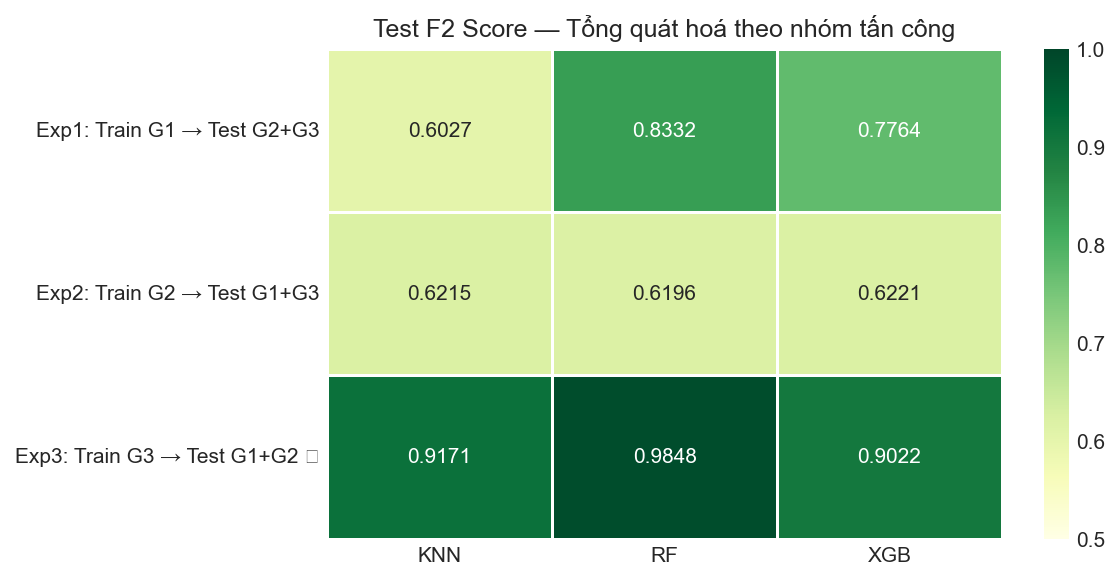
\includegraphics[width=\linewidth]{hinh/phase2_heatmap.png}
    \caption{Heatmap Test F2 theo thí nghiệm và mô hình.}
    \label{fig:phase2_heatmap}
\end{figure}

Heatmap cho thấy bất đối xứng rõ rệt giữa ba thí nghiệm: Exp 3 nổi bật ở góc phải trên, trong khi Exp 1 và Exp 2 đồng loạt thấp, gợi ý vấn đề tổng quát hóa xuất phát từ đặc tính của nhóm huấn luyện chứ không phải từ mô hình cụ thể.

Hình~\ref{fig:phase2_roc} thể hiện đường cong ROC trên tập test cho từng thí nghiệm.

\begin{figure}[H]
    \centering
    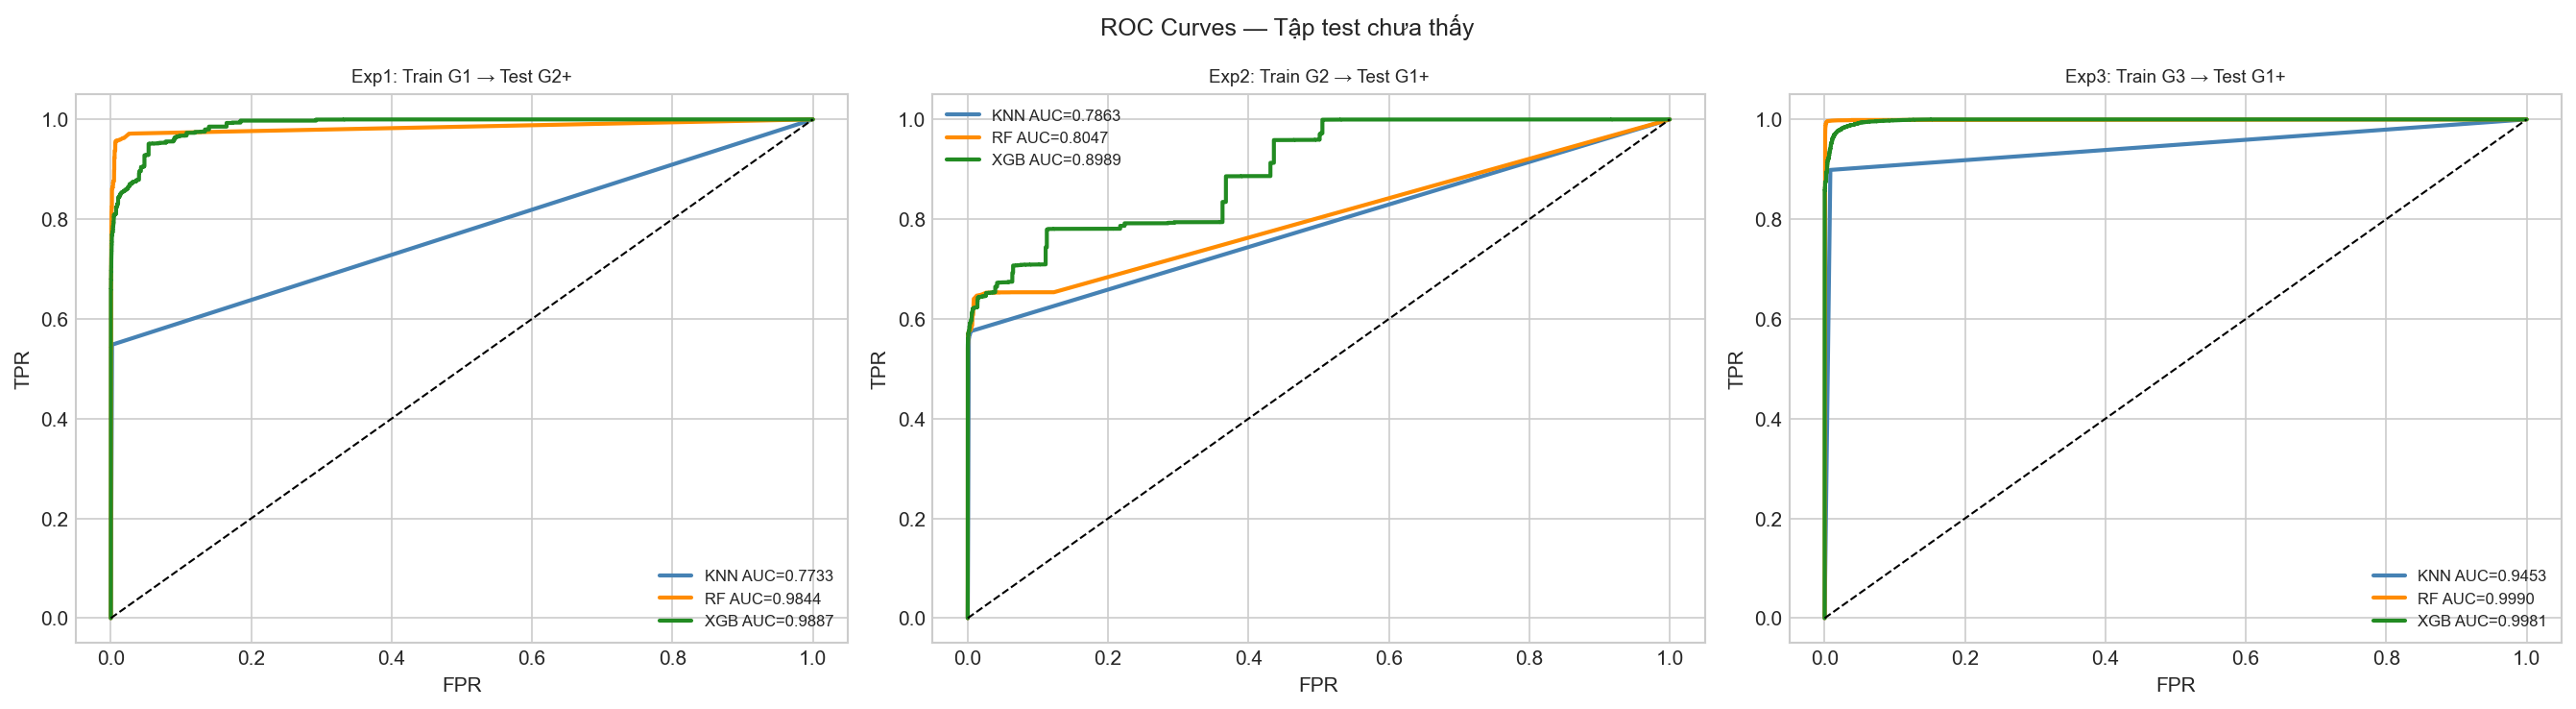
\includegraphics[width=\linewidth]{hinh/phase2_roc.png}
    \caption{Đường cong ROC trên tập test.}
    \label{fig:phase2_roc}
\end{figure}

Đường cong ROC tách biệt rõ Exp 3 (góc trên trái) so với Exp 1/2, xác nhận rằng sự suy giảm Test F2 phản ánh giới hạn hệ thống chứ không phải do ngưỡng phân loại. KNN ở Exp 1 và Exp 2 có AUC thấp nhất ($\approx$ 0,77--0,80), cho thấy bản thân xác suất phân loại cũng kém tin cậy ở những kịch bản này.

Hình~\ref{fig:phase2_confusion} thể hiện ma trận nhầm lẫn của mô hình tốt nhất mỗi thí nghiệm.

\begin{figure}[H]
    \centering
    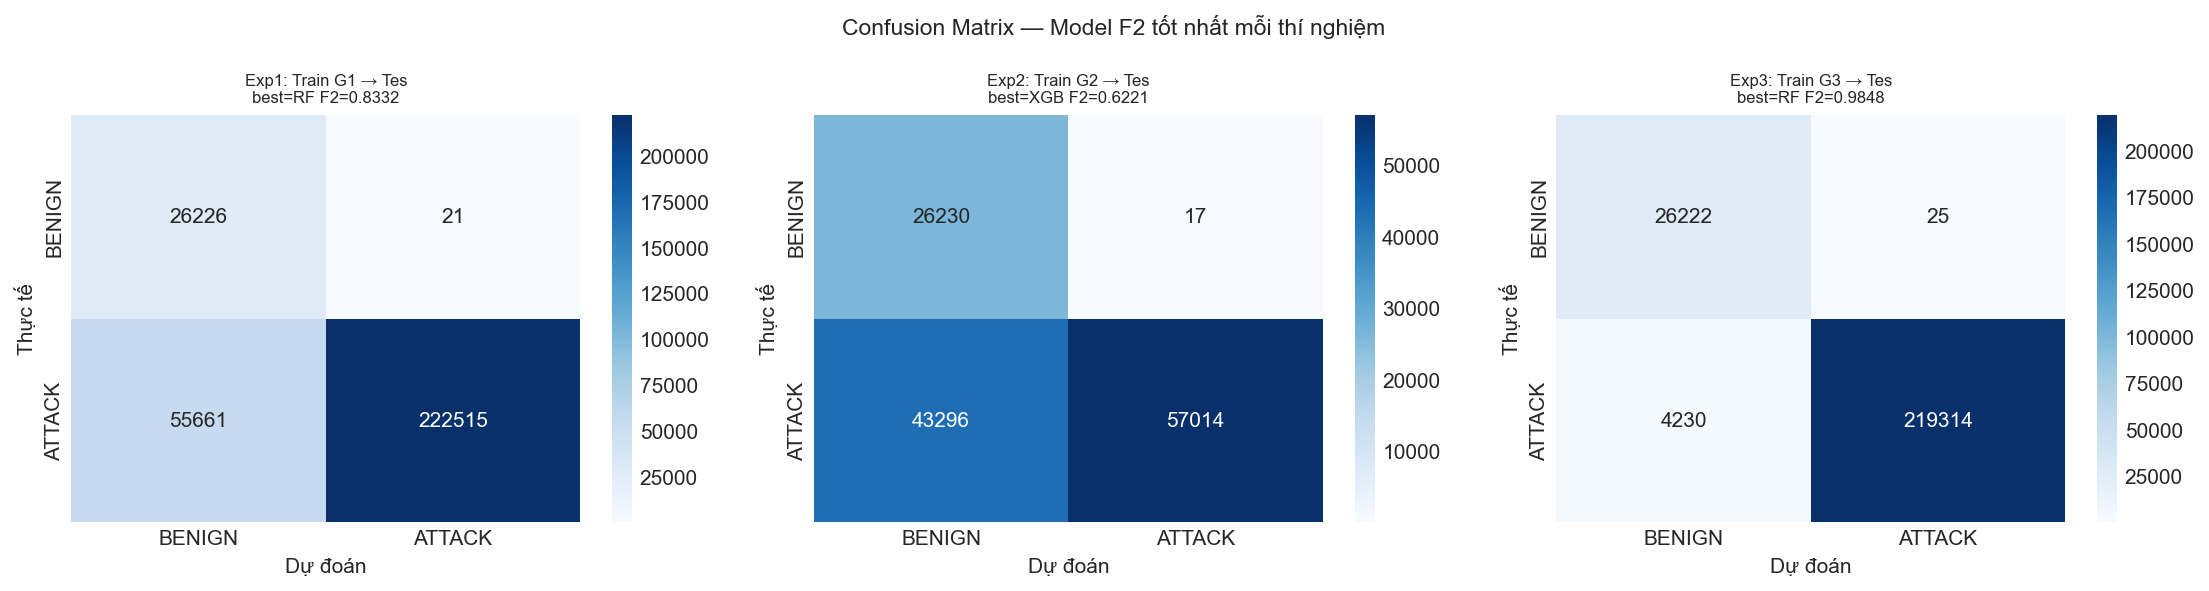
\includegraphics[width=\linewidth]{hinh/phase2_confusion_matrix.png}
    \caption{Ma trận nhầm lẫn của mô hình tốt nhất mỗi thí nghiệm.}
    \label{fig:phase2_confusion}
\end{figure}

Ma trận nhầm lẫn làm nổi bật nguồn gốc lỗi: ở Exp 1\&2, phần lớn lỗi là False Negative (tấn công bị phân loại là Benign), trái với Exp 3 nơi cả hai loại lỗi đều gần bằng không. Điều này xác nhận rằng mô hình không học được biên phân tách tổng quát khi tập huấn luyện đơn điệu về giao thức.

Hình~\ref{fig:phase2_cv_boxplot} thể hiện phân phối CV F2 qua 5 fold cho từng thí nghiệm.

\begin{figure}[H]
    \centering
    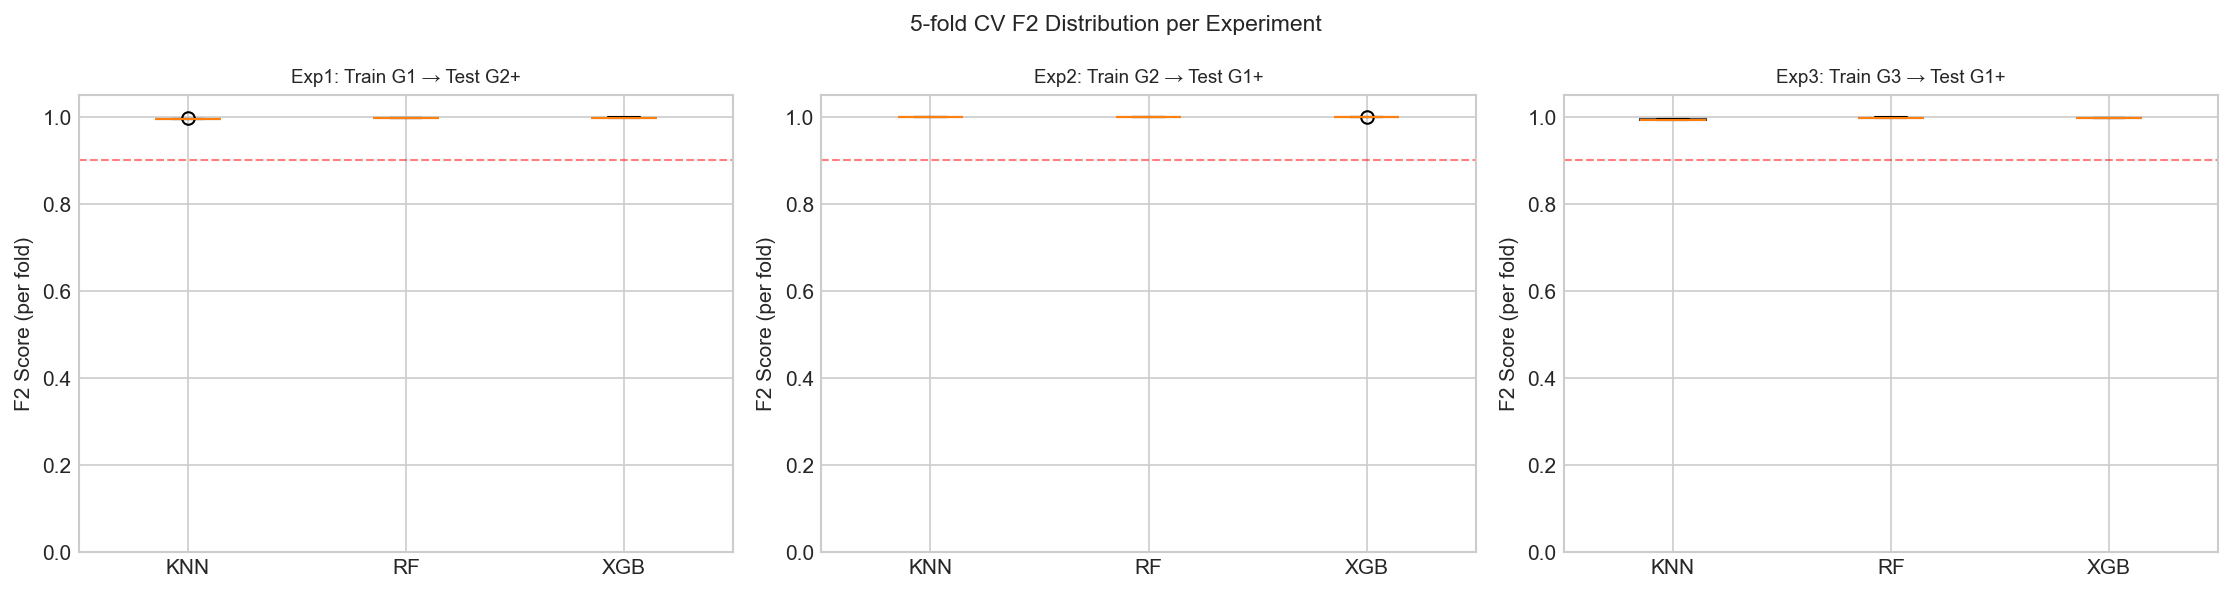
\includegraphics[width=\linewidth]{hinh/phase2_cv_boxplot.png}
    \caption{Phân phối CV F2 qua 5 fold theo từng thí nghiệm.}
    \label{fig:phase2_cv_boxplot}
\end{figure}

CV F2 rất ổn định (độ lệch chuẩn nhỏ) ở cả ba thí nghiệm, xác nhận rằng Gap lớn ở Exp 1\&2 xuất phát từ overfitting nhóm tấn công, không phải từ sự bất ổn của quá trình cross-validation.

Hình~\ref{fig:phase2_feature_importance} thể hiện feature importance của RF và XGB.

\begin{figure}[H]
    \centering
    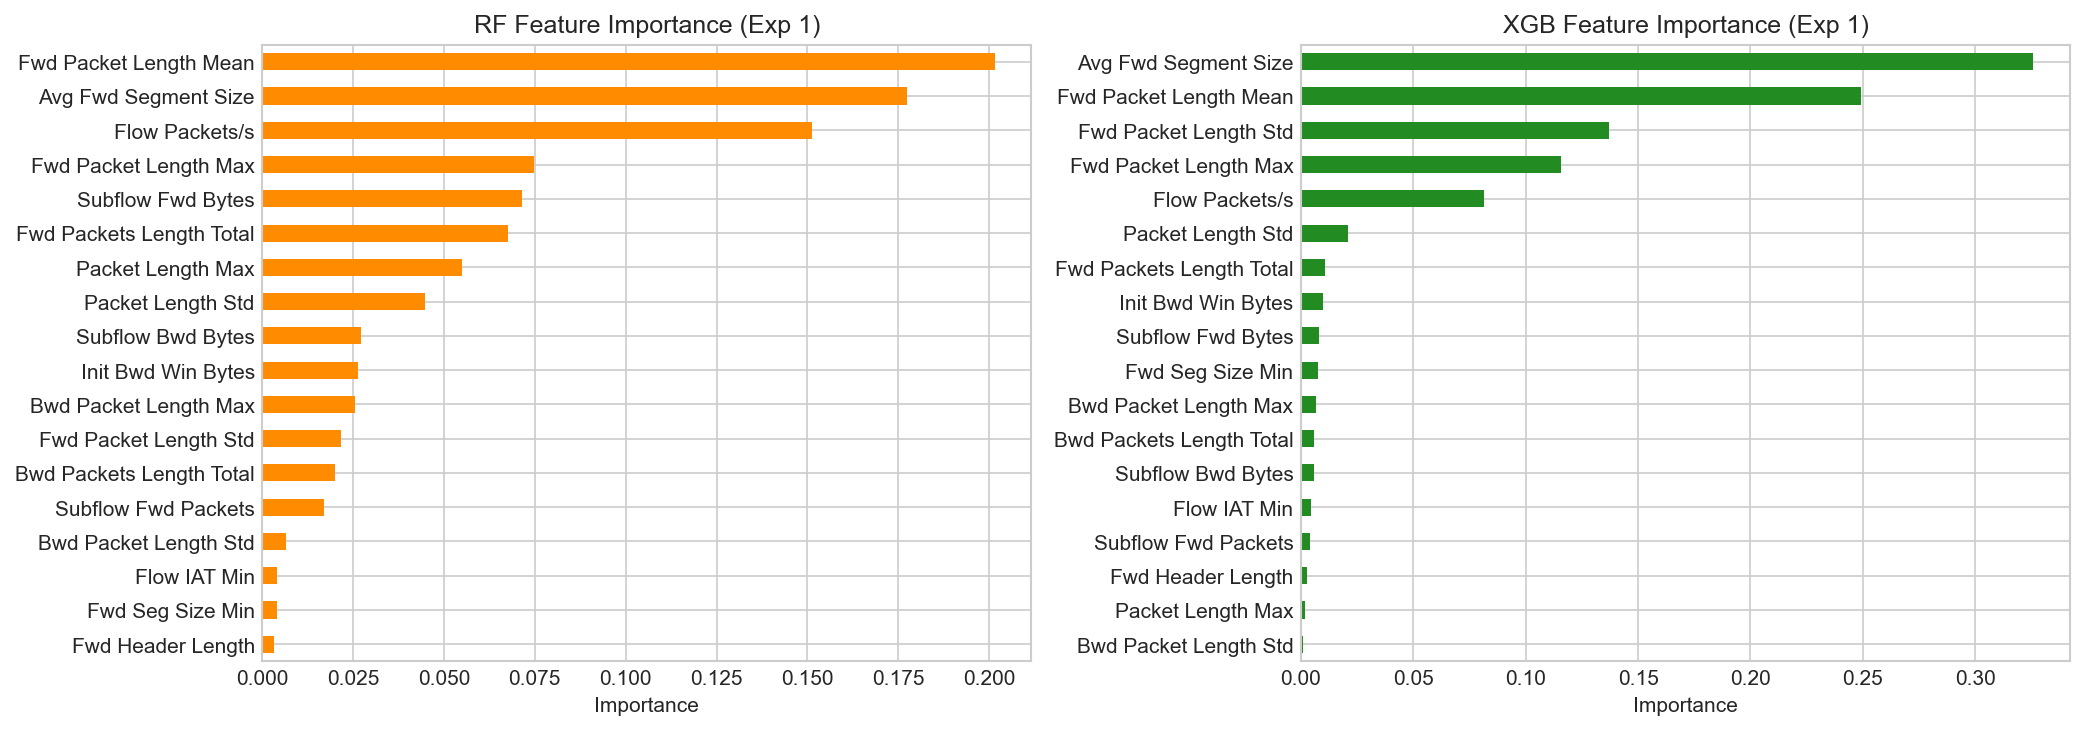
\includegraphics[width=\linewidth]{hinh/phase2_feature_importance.png}
    \caption{Feature importance của RF và XGB.}
    \label{fig:phase2_feature_importance}
\end{figure}

Các đặc trưng thể tích như \texttt{Fwd Packet Length Mean/Max}, \texttt{Flow IAT Max}, \texttt{Flow Bytes/s} chiếm tỷ trọng lớn trong cả RF và XGB, phù hợp với lý giải về sự tương đồng giữa G3 và bộ dữ liệu Kaggle.

Hình~\ref{fig:phase2_optuna_history} thể hiện lịch sử tối ưu Optuna theo số trial.

\begin{figure}[H]
    \centering
    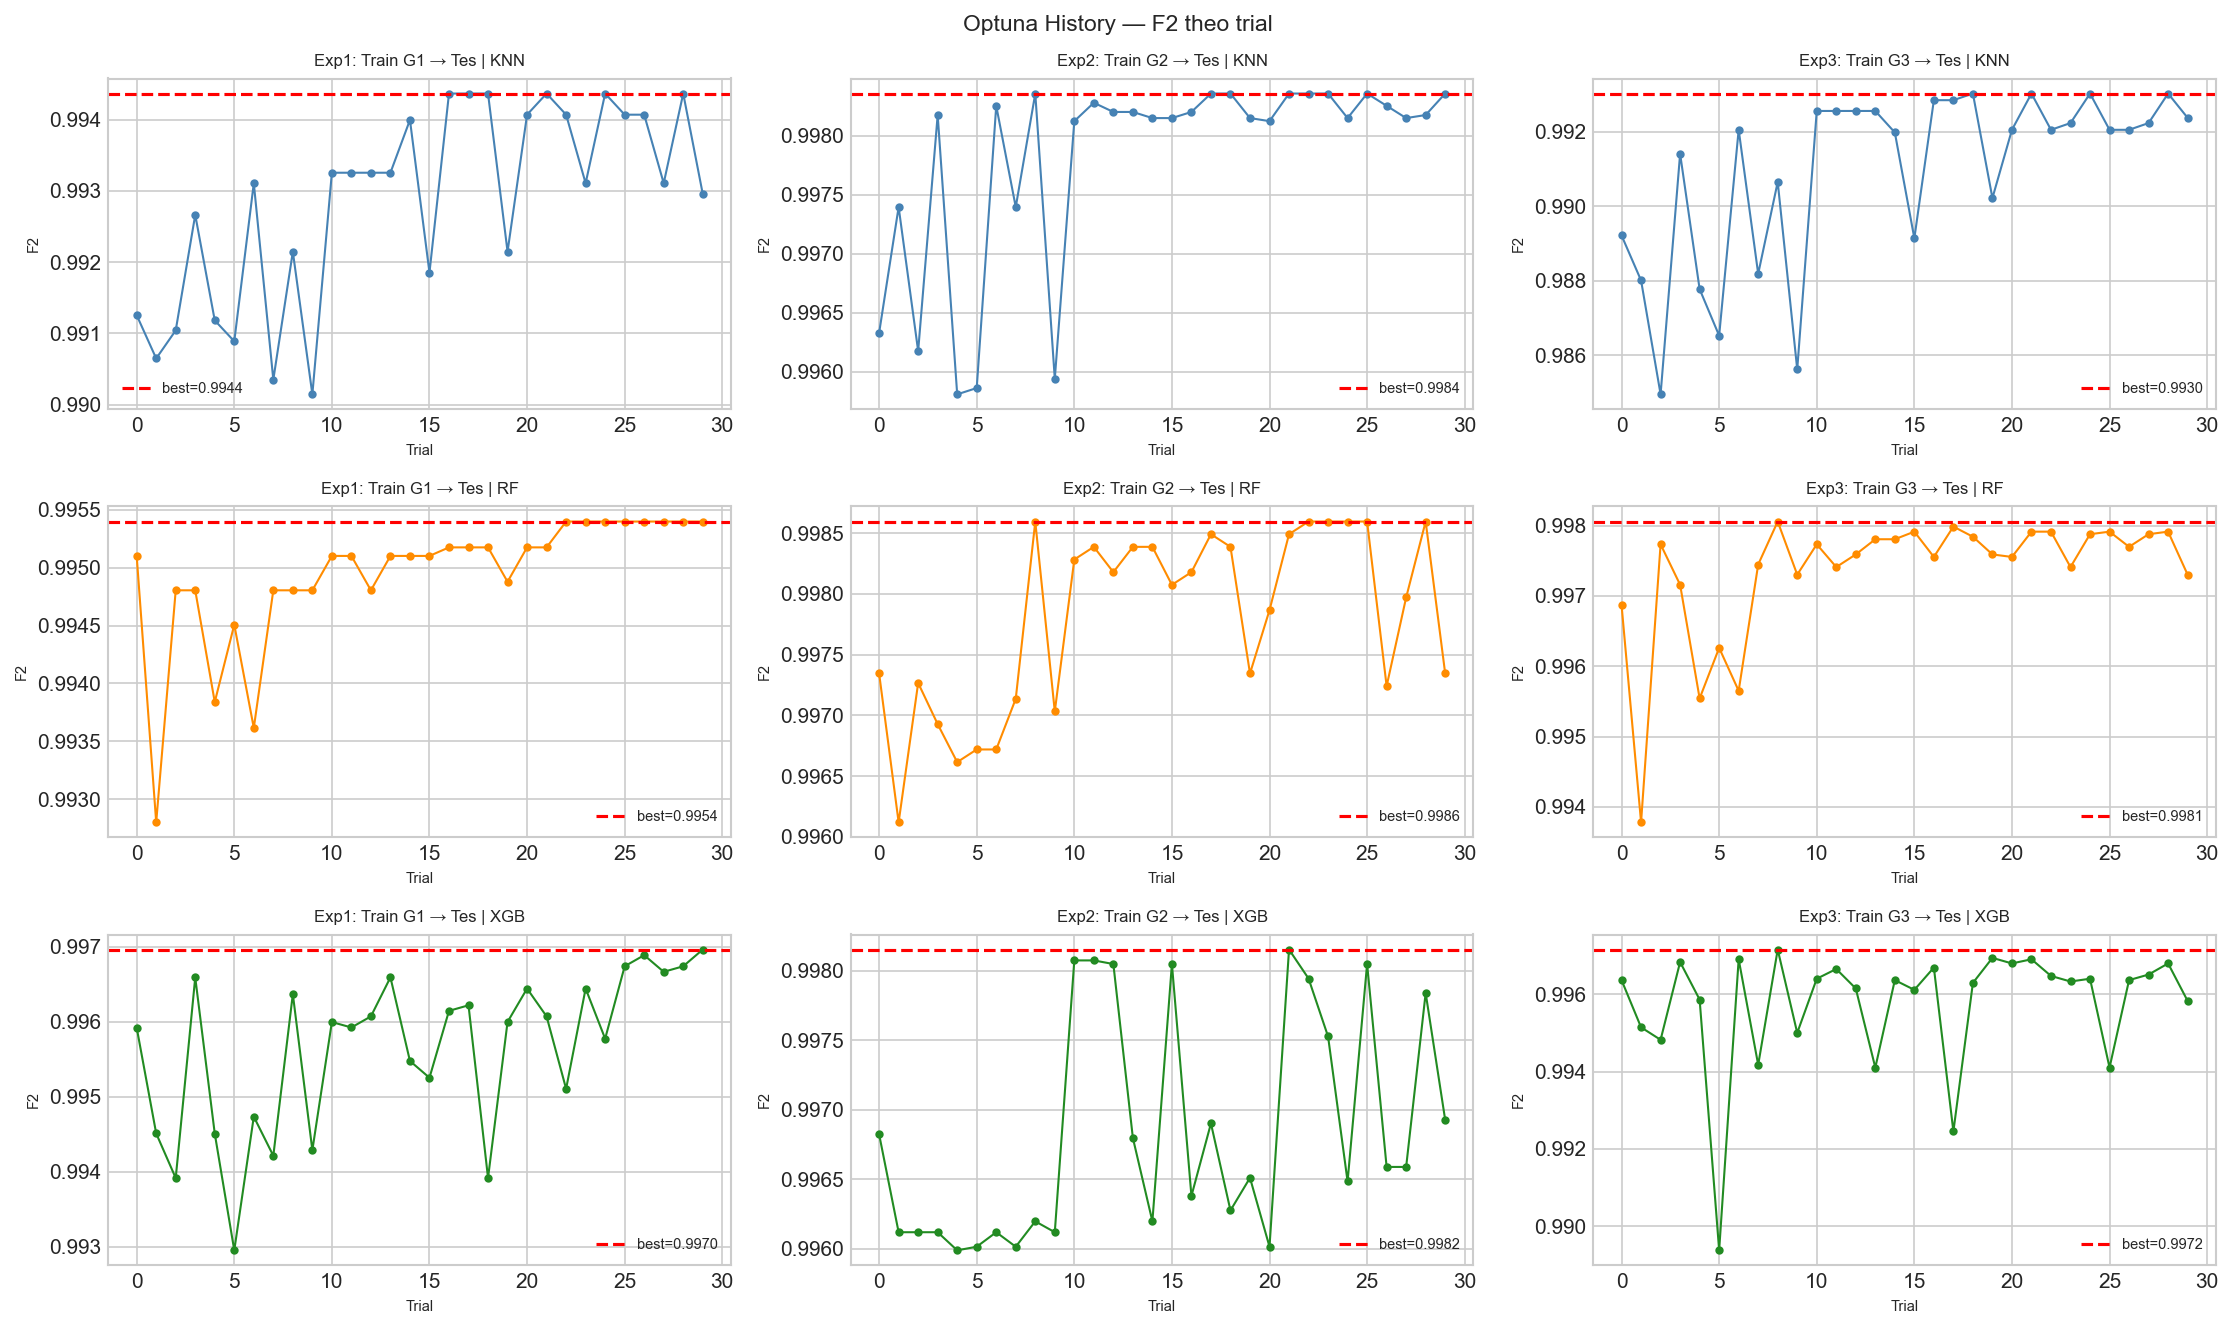
\includegraphics[width=\linewidth]{hinh/phase2_optuna_history.png}
    \caption{Lịch sử tối ưu Optuna theo số trial.}
    \label{fig:phase2_optuna_history}
\end{figure}

Optuna TPE hội tụ nhanh, thường tìm được siêu tham số tốt sau 10--15 trong tổng số 30 trial ở cả ba thí nghiệm.

Bảng~\ref{tab:optuna_params} liệt kê bộ siêu tham số tốt nhất mà Optuna tìm được cho từng mô hình và từng thí nghiệm.

\begin{table*}[!t]
\caption{Siêu tham số tốt nhất do Optuna TPE tìm được (30 trial, subsample 50.000 mẫu/trial). KNN cố định \texttt{algorithm=ball\_tree}; các tham số còn lại do Optuna tối ưu.}
\label{tab:optuna_params}
\begin{center}
\begin{adjustbox}{width=\textwidth}
\begin{tabular}{|l|l|l|}
\hline
\textbf{Thí nghiệm} & \textbf{Mô hình} & \textbf{Siêu tham số tốt nhất} \\
\hline
\multirow{3}{*}{Exp 1 (G1)} & KNN & \texttt{n\_neighbors=3, weights=distance} \\
 & RF  & \texttt{n\_estimators=100, max\_depth=19, min\_samples\_split=2, max\_features=log2} \\
 & XGB & \texttt{n\_estimators=500, max\_depth=7, learning\_rate=0.035, subsample=0.785, colsample\_bytree=0.744} \\
\hline
\multirow{3}{*}{Exp 2 (G2)} & KNN & \texttt{n\_neighbors=5, weights=distance} \\
 & RF  & \texttt{n\_estimators=150, max\_depth=18, min\_samples\_split=2, max\_features=log2} \\
 & XGB & \texttt{n\_estimators=450, max\_depth=7, learning\_rate=0.094, subsample=0.999, colsample\_bytree=0.816} \\
\hline
\multirow{3}{*}{Exp 3 (G3)} & KNN & \texttt{n\_neighbors=3, weights=distance} \\
 & RF  & \texttt{n\_estimators=500, max\_depth=15, min\_samples\_split=5, max\_features=log2} \\
 & XGB & \texttt{n\_estimators=200, max\_depth=6, learning\_rate=0.133, subsample=0.918, colsample\_bytree=0.820} \\
\hline
\end{tabular}
\end{adjustbox}
\end{center}
\end{table*}

\subsection{Đánh giá hiệu quả tính toán}

Một trong những mục tiêu quan trọng của bước lựa chọn đặc trưng FAMS là giảm số chiều đầu vào của mô hình, từ đó rút ngắn thời gian huấn luyện và suy luận. Bảng~\ref{tab:timing} trình bày thời gian huấn luyện và thời gian suy luận của ba mô hình trên ba thí nghiệm.

Về mặt lý thuyết, việc giảm từ 70+ đặc trưng xuống còn 18 đặc trưng (giảm $\approx$75\% số chiều) có tác động khác nhau tùy mô hình:
\begin{itemize}
    \item \textbf{KNN:} Hưởng lợi nhiều nhất vì chi phí suy luận tỷ lệ trực tiếp với số chiều $d$ -- tính khoảng cách Euclid trên 18 chiều nhanh hơn đáng kể so với 70+ chiều.
    \item \textbf{Random Forest \& XGBoost:} Giảm số chiều giúp rút ngắn thời gian tìm điểm chia tại mỗi nút cây, qua đó giảm thời gian huấn luyện; tác động đến suy luận ít hơn KNN nhưng vẫn có ý nghĩa khi tập test lớn.
\end{itemize}

\begin{table}[H]
\caption{Thời gian huấn luyện (s) và suy luận (ms/mẫu) của các mô hình theo từng thí nghiệm. KNN sử dụng \texttt{algorithm=ball\_tree} cố định để đảm bảo so sánh nhất quán.}
\label{tab:timing}
\begin{center}
\begin{adjustbox}{width=\linewidth}
\begin{tabular}{|l|l|r|r|r|r|}
\hline
\textbf{Thí nghiệm} & \textbf{Mô hình} & \textbf{Train size} & \textbf{T. huấn luyện (s)} & \textbf{T. suy luận (ms/mẫu)} & \textbf{Test F2} \\
\hline
Exp 1 (G1$\to$G2+G3) & KNN & 124.225 & 0,06 & 0,1102 & 0,5790 \\
                      & RF  & 124.225 & 1,00 & 0,0031 & 0,8330 \\
                      & XGB & 124.225 & 1,96 & 0,0013 & 0,7753 \\
\hline
Exp 2 (G2$\to$G1+G3) & KNN & 318.116 & 0,20 & 0,1526 & 0,5741 \\
                      & RF  & 318.116 & 2,53 & 0,0054 & 0,6032 \\
                      & XGB & 318.116 & 2,62 & 0,0009 & 0,6058 \\
\hline
Exp 3 (G3$\to$G1+G2) & KNN & 184.692 & 0,09 & 0,0559 & 0,9204 \\
                      & RF  & 184.692 & 5,73 & 0,0111 & 0,9870 \\
                      & XGB & 184.692 & 0,83 & 0,0005 & 0,9519 \\
\hline
\end{tabular}
\end{adjustbox}
\end{center}
\end{table}

\subsection{Tổng hợp và nhận xét}

\subsubsection{So sánh ba mô hình}

\textbf{Random Forest} là mô hình nhất quán nhất về khả năng tổng quát hóa: đạt Test F2 cao nhất ở Exp 1 (0,83) và Exp 3 (0,98), đồng thời có Gap nhỏ nhất ở Exp 3 (+0,013). Cơ chế bagging của RF giúp giảm phương sai và tránh overfit vào đặc trưng đặc thù của nhóm tấn công huấn luyện.

\textbf{XGBoost} đạt AUC cao (0,99 ở Exp 1 và Exp 3) nhưng có Gap lớn hơn RF ở Exp 3 (+0,096 so với +0,013). Điều này gợi ý XGBoost có xu hướng học các pattern phức tạp hơn của tập train, nhưng phần pattern đó không hoàn toàn chuyển giao sang nhóm tấn công mới.

\textbf{KNN} có Test F2 thấp nhất ở Exp 1 và Exp 2 (khoảng 0,61), nhưng cải thiện lên 0,92 ở Exp 3. Điều này phù hợp với đặc tính của KNN: hoạt động tốt khi phân phối dữ liệu train và test có sự tương đồng cao trong không gian đặc trưng (trường hợp Exp 3), nhưng kém khi phân phối khác biệt lớn.

\subsubsection{Ảnh hưởng của đặc trưng FAMS đến tổng quát hóa}

Kết quả thực nghiệm cho thấy tập 18 đặc trưng FAMS được tối ưu hóa cho bộ dữ liệu Kaggle (chứa nhiều tấn công thể tích như UDP Flood, Syn) phù hợp tốt hơn với G3 (Exploitation) so với G1/G2 (Reflection). Điều này dẫn đến bất đối xứng rõ rệt: tổng quát hóa tốt từ G3 sang G1+G2 (Exp 3), nhưng kém từ G1 hay G2 sang các nhóm còn lại (Exp 1, Exp 2). Hiện tượng này là minh chứng cụ thể cho tầm quan trọng của sự phù hợp giữa phân phối dữ liệu lựa chọn đặc trưng và dữ liệu huấn luyện mô hình trong một pipeline hai giai đoạn.

\subsubsection{Trả lời câu hỏi nghiên cứu}

Dựa trên kết quả thực nghiệm, ba câu hỏi nghiên cứu đặt ra trong Chương~\ref{sec:gioi-thieu} được trả lời như sau:

\begin{enumerate}
    \item \textbf{Tập đặc trưng FAMS từ Kaggle có hiệu quả trên CIC-DDoS 2019 không?} -- \textit{Có, nhưng không đồng đều.} Tập 18 đặc trưng đạt Test F2 = 0,98 (RF, Exp 3) khi nhóm huấn luyện có đặc trưng tương đồng với Kaggle (Exploitation). Tuy nhiên, hiệu quả giảm rõ rệt (Test F2 = 0,60--0,83) khi nhóm huấn luyện là Reflection, phản ánh sự bất đối xứng giữa phân phối đặc trưng của hai bộ dữ liệu.

    \item \textbf{Mô hình huấn luyện trên một nhóm có tổng quát hóa tốt sang nhóm chưa thấy không?} -- \textit{Phụ thuộc vào tính đa dạng của nhóm huấn luyện.} G3 (Exploitation: Syn, UDP, UDPLag, WebDDoS) tổng quát hóa tốt sang G1+G2 với Gap $\approx$ 0,01. Ngược lại, G1 và G2 -- mỗi nhóm đặc trưng bởi một cơ chế giao thức hẹp -- tổng quát hóa kém với Gap = 0,16--0,39.

    \item \textbf{Mô hình nào tổng quát hóa tốt nhất theo Leave-One-Group-Out?} -- \textbf{Random Forest} nhất quán đạt Test F2 và Gap tốt nhất qua cả ba thí nghiệm, nhờ cơ chế bagging giảm phương sai và tránh overfit vào đặc trưng giao thức đặc thù. XGBoost có AUC cao nhưng Gap lớn hơn RF; KNN phụ thuộc nhiều vào sự tương đồng phân phối train/test.
\end{enumerate}

\subsubsection{Ý nghĩa thực tiễn}

Kết quả của thiết kế Leave-One-Group-Out có ý nghĩa thực tiễn rõ rệt: trong triển khai thực tế, hệ thống phát hiện DDoS thường gặp các kiểu tấn công mới chưa có trong tập huấn luyện. Việc huấn luyện trên nhóm tấn công \textit{đa dạng} (như G3, bao gồm cả tấn công thể tích lẫn tầng ứng dụng) tạo ra mô hình tổng quát hóa tốt hơn so với huấn luyện trên nhóm đơn điệu (như G2 chỉ có NTP/TFTP). Điều này gợi ý rằng chiến lược thu thập dữ liệu huấn luyện cần ưu tiên \textit{đa dạng loại tấn công} hơn là \textit{số lượng mẫu thuần túy}.
